\documentclass[a4paper,twoside,bibtotoc,abstracton,12pt,BCOR=15mm]{article}
\usepackage[english]{babel}
\usepackage[utf8]{inputenc}
\usepackage{graphicx}
\usepackage{booktabs}
\usepackage[table]{xcolor}
\usepackage{colortbl}
\usepackage{color}
\usepackage{graphicx}
\usepackage{makeidx}  % allows for indexgeneration
\usepackage{amsmath, amssymb} % amsthm stuff also defined by llncs
\usepackage{graphicx}
\usepackage{subfig} 
\usepackage{url}
\usepackage{color}
\usepackage{booktabs}
\usepackage{listings}
\usepackage{xspace}
\usepackage{lscape}
\usepackage{listings}
\usepackage{color}

\graphicspath{{.}{../Common/}{../../Common/}}

\def\deliverableNumber{8.4.1}
\def\deliverableTitle{Online Collaboration Platform}

\def\disseminationLevel{Public}
\def\dueDate{Month 6, 28/2/2011}
\def\submissionDate{02/3/2011}
\def\workPackage{WP8,Project Management}
\def\task{Task T8.4}
\def\type{Report}
\def\approvalStatus{Approved}
\def\version{1.0}
\def\numberOfPages{67}
\def\filename{D8.4.1\_Online\_Collaboration\_Platform\_Public.pdf}

\definecolor{lod_blue}{RGB}{192,227,242}
\definecolor{LodBlue}{rgb}{0.7529,0.8902,0.9490}

\newcommand{\orchid}{\textsc{Orchid}\xspace}
\newcommand{\geolift}{\textsc{GeoLift}\xspace}
\newcommand{\limes}{\textsc{Limes}\xspace}
\DeclareMathOperator*{\argmax}{arg\,max}
\DeclareMathOperator*{\argmin}{arg\,min}

%%%%%%%%%%%%%%%%%%%%%%%%%%%%%%%%%%%%%%%%%%%%%%%%%%%%%%%%%%%%%%%%%%%%%%%%%%%%%%%%%%
\definecolor{dkgreen}{rgb}{0,0.6,0}
\definecolor{gray}{rgb}{0.5,0.5,0.5}
\definecolor{mauve}{rgb}{0.58,0,0.82}

\lstset{frame=tb,
  language=Java,
  aboveskip=3mm,
  belowskip=3mm,
  showstringspaces=false,
  columns=flexible,
  basicstyle={\small\ttfamily},
  numbers=none,
  numberstyle=\tiny\color{gray},
  keywordstyle=\color{blue},
  commentstyle=\color{dkgreen},
  stringstyle=\color{mauve},
  breaklines=true,
  breakatwhitespace=true
  tabsize=3
}
%%%%%%%%%%%%%%%%%%%%%%%%%%%%%%%%%%%%%%%%%%%%%%%%%%%%%%%%%%%%%%%%%%%%%%%%%%%%%%%%%%
\begin{document}



%\small{ Making the Web an Exploratory for Geospatial Knowledge}


\vspace*{\fill} 
\begin{quote} 
\centering 
\begin{center}
 
\includegraphics[scale=0.5]{images/geoknow.png}
\end{center}
\begin{flushleft}
 \Large{\geolift}
 \small{ - Spatial mapping framework for enriching RDF datasets with Geo-spatial information.}
\end{flushleft}
\end{quote}
\vspace*{\fill}
\newpage

\vspace*{\fill} 
\begin{quote} 

\textbf{Abstract}: \\
This manual presents the spatial mapping component dubbed \geolift. 
The goal of \geolift is to enrich RDF datasets with geo-spatial information. 
To achieve this goal, GeoLit relies on three atomic modules based on dereferencing, linking and NLP. 
\geolift was implemented in Java, is open-source and can be accessed at \url{https://github.com/GeoKnow/GeoLift/}. 
\end{quote}
\vspace*{\fill}

\newpage
\tableofcontents
\newpage

\section{Introduction}
Manifold RDF data contain implicit references to geographic data.
For example, music datasets such as \emph{Jamendo} include references to locations of record labels, places where artists were born or have been, etc.
The aim of the spatial mapping component, dubbed \geolift, is to retrieve this information and make it explicit.
In the following, we begin by presenting the basic assumptions that influence the development of the first component of \geolift.
Then, we present the technical approach behind \geolift.
Finally, we present the detailed developers' manual of \geolift.
%in which we introduce how to deal with different modules of \geolift and integrate it with other tool.

\section{Assumptions}
Geographical information can be mentioned in three different ways within Linked Data:
\begin{enumerate}
\item \emph{Through dereferencing}: Several datasets contain links to datasets with explicit geographical information such as \emph{DBpedia} or \emph{LinkedGeoData}. 
For example, in a music dataset, one might find information such as\\ 
\texttt{http://example.org/Leipzig \\
owl:sameAs \\ 
http://dbpedia.org/resource/Leipzig}.

We call this type of reference \emph{explicit}. 
We can now use the semantics of RDF to fetch geographical information from DBpedia and attach it to the resource in the other ontology as \texttt{http://example.org/Leipzig} and \texttt{http://dbpedia.org/resource/Leipzig} refer to the same real-world object.

\item \emph{Through linking}: It is known that the Web of Data contains an insufficient number of links. 
The latest approximations suggest that the Linked Open Data Cloud alone consists of 31+ billion triples but only contains approximately 0.5 billion links (i.e., less than 2\% of the triples are links between knowledge bases). 
The second intuition behind our approach is thus to use link discovery to map resources in an input knowledge base to resources in a knowledge that contains explicit geographical information. 
For example, given a resource \texttt{http://example.org/Athen}, \geolift should aim to find a resource such as \texttt{http://dbpedia.org/resource/Athen} to map it with. 
Once having established the link between the two resources, \geolift can then resolve to the approach defined above.

\item \emph{Through Natural Language Processing}: In some cases, the geographic information is hidden in the objects of data type properties. 
For example, some datasets contain biographies, textual abstracts describing resources, comments from users, etc.
The idea here is to use this information by extracting Named Entities and keywords using automated Information Extraction techniques.
Semantic Web Frameworks such as FOX\footnote{\url{http://fox.aksw.org}} have the main advantage of providing URIs for the keywords and entities that they detect.
These URIs can finally be linked with the resources to which the datatype properties were attached.
Finally, the geographical information can be dereferenced and attached to the resources whose datatype properties were analyzed.
\end{enumerate}

The idea behind \geolift is to provide a generic architecture that contains means to exploit these three characteristics of Linked Data. 
In the following, we present the technical approach underlying \geolift.

\section{Technical Approach}
\subsection{Architecture}
\geolift was designed to be a modular tool which can be easily extended and re-purposed.
In its first version, it provides two main types of artifacts:
\begin{enumerate}
\item \emph{Modules}: These artifacts are in charge of generating geographical data based on RDF data. 
To this aim, they implement the three intuitions presented above.
The input for such a module is an RDF dataset (in Java, a \emph{Jena Model}).
The output is also an RDF dataset enriched with geographical information (in Java, an enriched \emph{Jena Model}).
Formally, a module can thus be regarded as a function $\mu: \mathcal{R} \rightarrow \mathcal{R}$, where $\mathcal{R}$ is the set of all RDF datasets.
\item \emph{Operators}: The idea behind operators is to enable users to define a workflow for processing their input dataset. 
Thus, in case a user knows the type of enrichment that is to be carried out (using linking and then links for example), he can define the sequence of modules that must be used to process his dataset.
Note that the format of the input and output of modules is identical. 
Thus, the user is empowered to create workflows of arbitrary complexity by simply connecting modules.
Formally, an operator can be regarded as a function $\varphi: \mathcal{R} \cup \mathcal{R}^2 \rightarrow \mathcal{R} \cup \mathcal{R}^2$.
\end{enumerate}
The corresponding architecture is shown in Figure~\ref{fig:architecture}. The input layer allows reading RDF in different serializations.
The enrichment modules are in the second layer and allow adding geographical information to RDF datasets by different means.
The operators (which will be implemented in the future version of \geolift) will combine the enrichment modules and allow defining a workflow for processing information.
The output layer serializes the results in different format.
The enrichment procedure will be monitored by implementing a controller, which will be added in the future version of \geolift.


\begin{figure}[ht!]
			\centering
			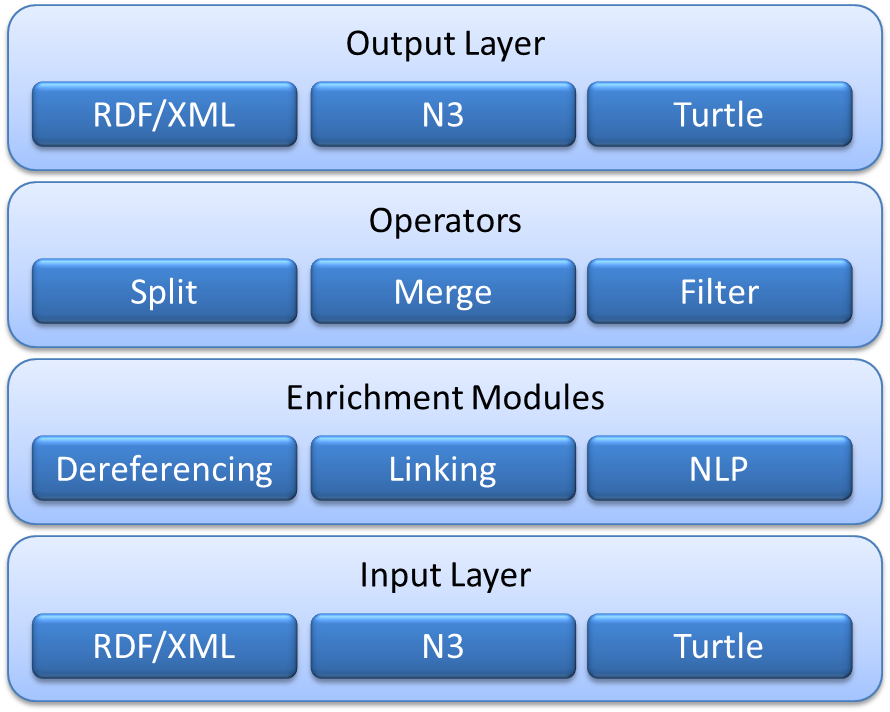
\includegraphics[width = 0.6\textwidth]{images/geolift_architecture.png}
			\caption{Architecture of \geolift}
			\label{fig:architecture}
		\end{figure}

In the following, we present the implementation of the three intuitions presented above in \geolift.
\subsection{Using Dereferencing}
For datasets which contain \texttt{owl:sameAs} links, we deference all links from the dataset to other datasets by using a content negotiation on HTTP as shown in Figure~\ref{fig:contentNegotiation}.
This returns a set of triples that needs to be filtered for relevant geographical information.
Here, we use a predefined list of attributes that links to geographical information.
Amongst others, we look for \texttt{geo:lat}, \texttt{geo:long}, \texttt{geo:lat\_long}, \texttt{geo:line} and \texttt{geo:polygon}.
The list of retrieved property values can be configured.

\begin{figure}[htb]
\centering
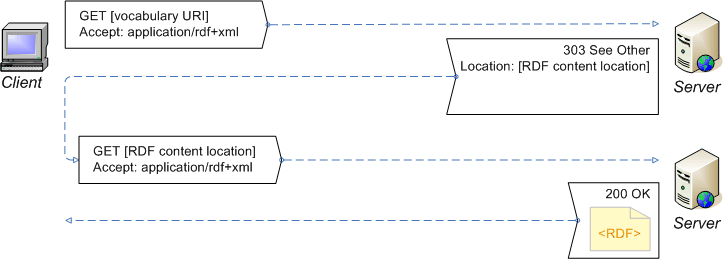
\includegraphics[width=0.7\textwidth]{images/contentnegotiation}
\caption{Content Negotiation as used by \geolift (courtesy of W3C)}
\label{fig:contentNegotiation}
\end{figure}

\subsection{Using Linking}
As pointed out before, links to geographical resources do not occur in several knowledge bases.
Here, we rely on the metrics implemented in the \limes framework\footnote{\url{http://\limes.sf.net}}~\cite{NGAU11,NGON12c,NGO+13c} to link the resources in the input dataset with geographical datasets.
\limes, the \textbf{Li}nk Discovery Framework for \textbf{Me}tric \textbf{S}paces, is a framework for discovering links between entities contained in Linked Data sources. \limes is a hybrid framework~\cite{NGON12c} that combines the mathematical characteristics of metric spaces as well prefix-, suffix- and position filtering to compute pessimistic approximations of the similarity of instances. These approximations are then used to filter out a large amount of those instance pairs that do not suffice the mapping conditions. By these means, \limes can reduce the number of comparisons needed during the mapping process by several orders of magnitude and complexity without loosing a single link.
The architecture of \limes is shown in Figure~\ref{fig:limesArchitecture}

\begin{figure}[ht!]
			\centering
			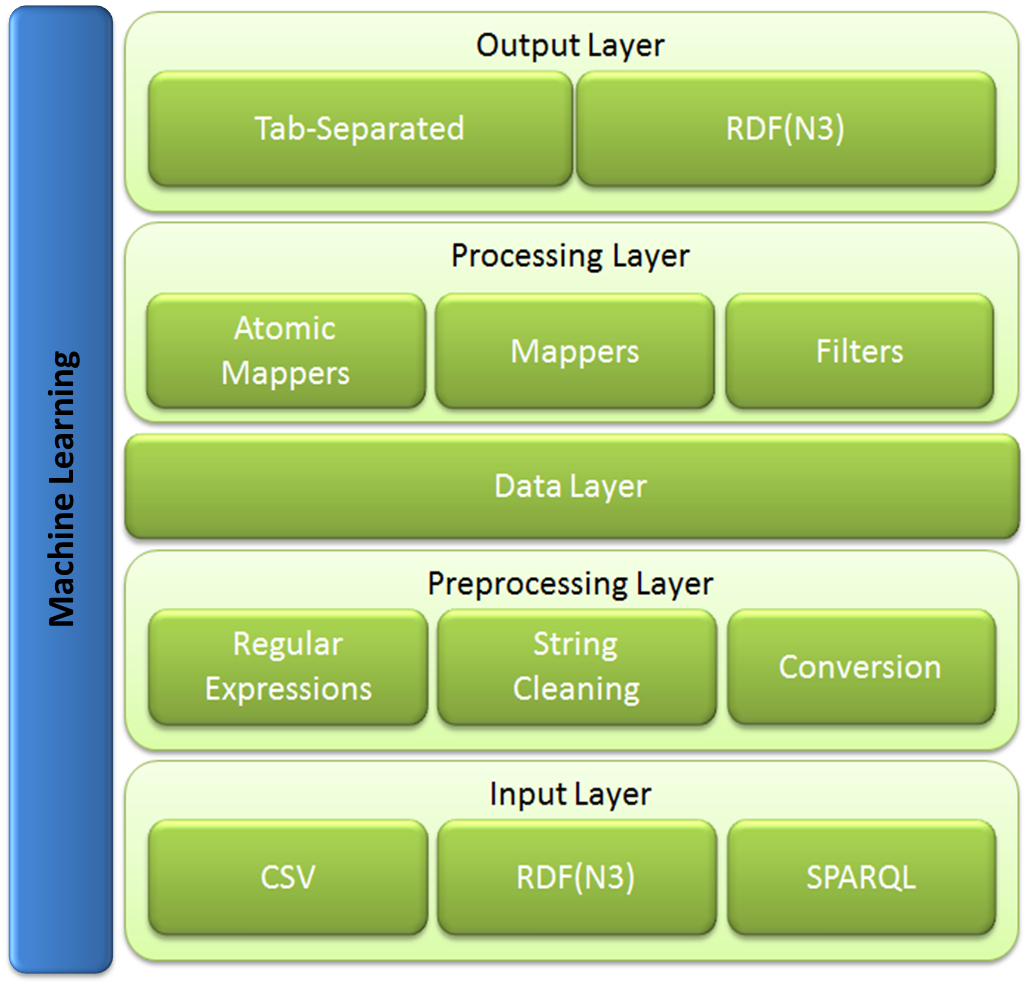
\includegraphics[width = 0.6\textwidth]{images/limesArchitecture.png}
			\caption{Architecture of \limes}
			\label{fig:limesArchitecture}
		\end{figure}
		


Linking using \limes~\cite{NGON12c,NGON12} can be achieved in three ways:
\begin{enumerate}
\item \emph{Manually}, by the means of a link specification~\cite{NGON12c}, which is an XML-description of (1) the resource in the input and target datasets that are to be linked and (2) of the similarity measure that is to employed to link these datasets.
\item \emph{Semi-automatically} based on active learning~\cite{NGO+11a,NGLY12,NGO+13b}. Here, the idea is that if the user is not an expert and thus unable to create a link specification, he can simply provide the framework with positive and negative examples iteratively. 
Based on these examples, \limes can compute links for mapping resources with high accuracy.
\item \emph{Automatically} based on unsupervised machine learning. Here, the user can simply specify the sets of resources that are to be linked with each other. 
\limes implements both a deterministic and non-deterministic machine-learning approaches that optimize a pseudo-F-measure to create a one-to-one mapping.
\end{enumerate}

The techniques implemented by \limes can be accessed via the SAIM user interface\footnote{\url{http://saim.aksw.org}}, of which a screenshot is shown in Figure~\ref{fig:saim_screenshot}.
\begin{figure}[htb]
\centering
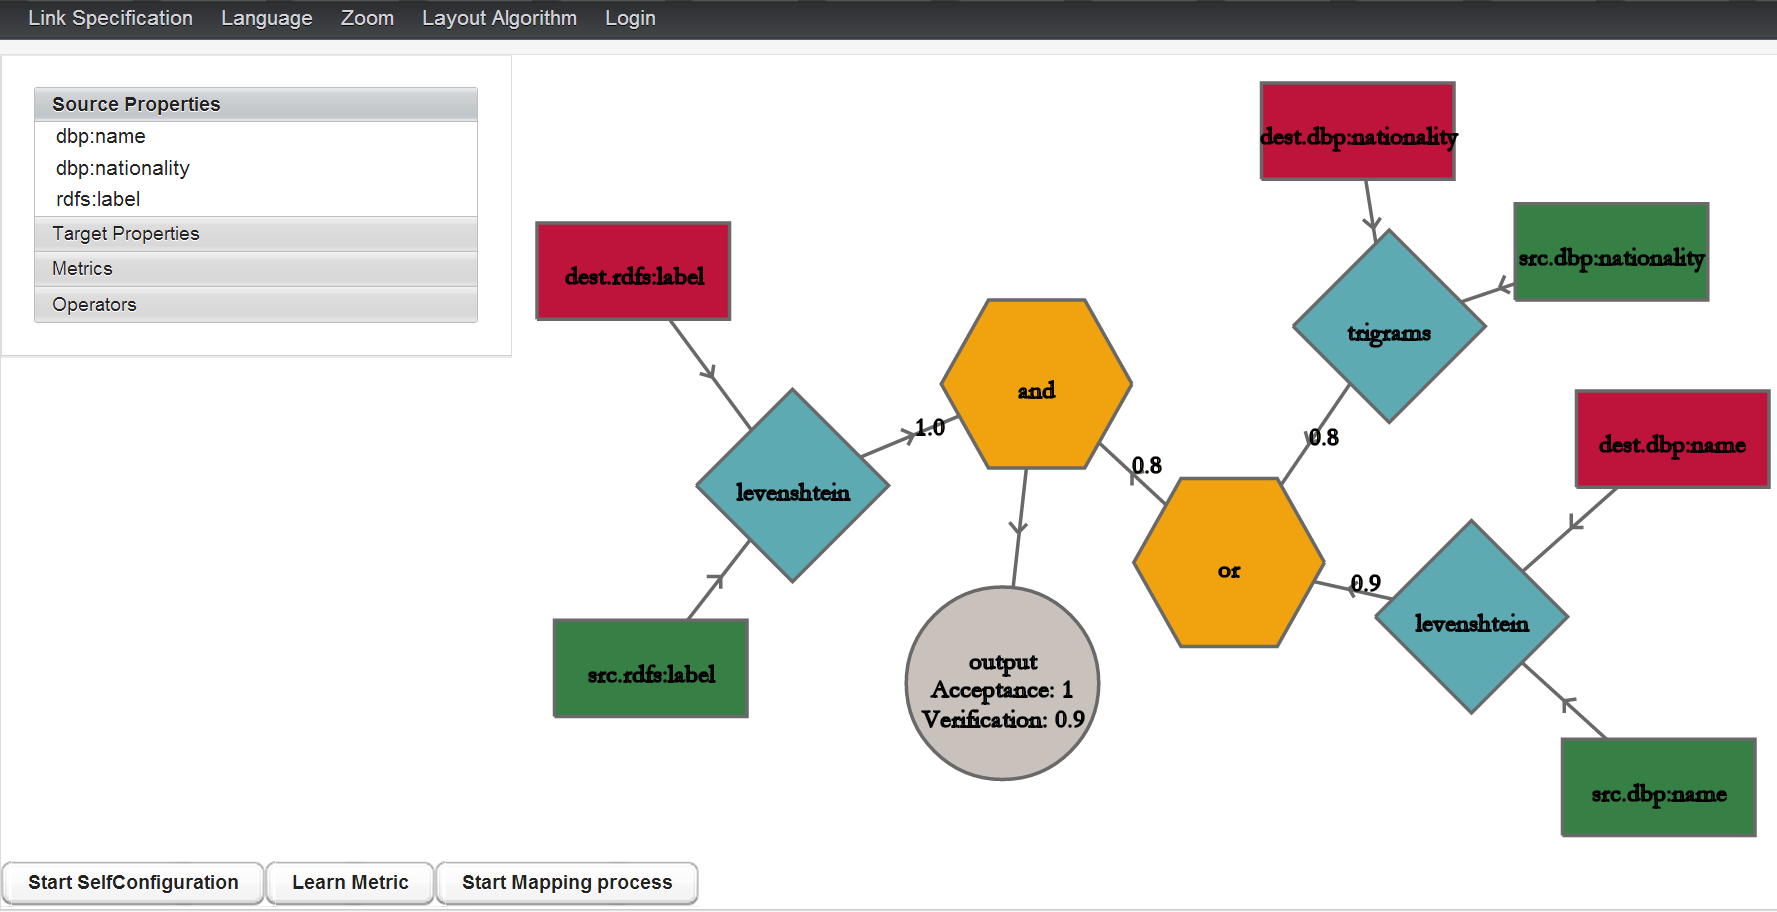
\includegraphics[width=0.7\textwidth]{images/saim_screenshot}
\caption{Screenshot of SAIM}
\label{fig:saim_screenshot}
\end{figure}

\subsection{Using Named Entity Recognition}
The geographical information hidden in datatype properties is retrieved by using Named Entity Recognition.
In the first version of \geolift, we rely on the FOX framework.
The FOX framework is a stateless and extensible framework that encompasses keyword extraction and named entity recognition. 
Its architecture consists of three layers as shown in Figure \ref{fig:foxArchitecture}.

\begin{figure}[htb]
\centering
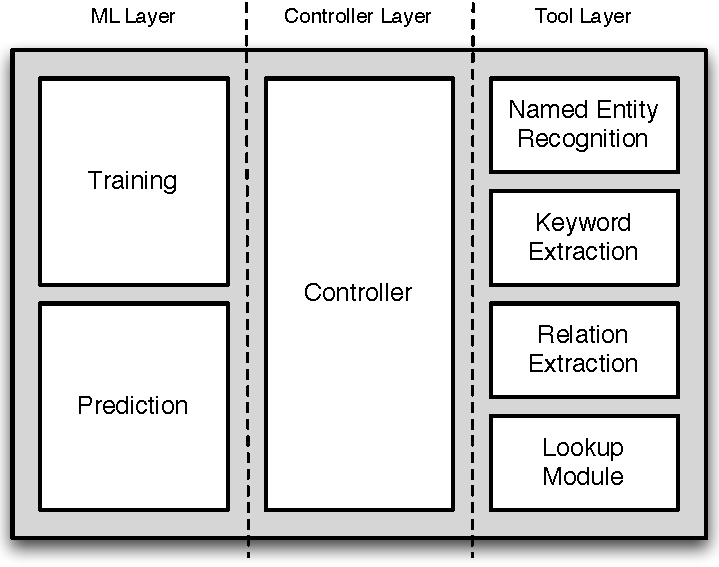
\includegraphics[width=0.55\textwidth]{images/FOX_Architecture}
\caption{Architecture of the FOX framework.}%
\label{fig:foxArchitecture}
\end{figure}

%The framework consists of three layers: a machine-learning layer, a controller layer and a tool layer.
FOX takes text or HTML as input.
Here we use the objects of datatype properties, i.e., plain text.
This data is sent to the \emph{controller layer}, which implements the functionality necessary to clean the data, i.e., remove HTML and XML tags as well as further noise.
Once the data has been cleaned, the controller layer begins with the orchestration of the tools in the \emph{tool layer}.
Each of the tools is assigned a thread from a thread pool, so as to maximize usage of multi-core CPUs.
Every thread runs its tool and generates an event once it has completed its computation.
In the event that a tool does not complete after a set time, the corresponding thread is terminated. 
So far, FOX integrates tools for KE, NER and RE. The KE is realized by tools such as KEA\footnote{\url{http://www.nzdl.org/Kea/}} and the Yahoo Term Extraction service\footnote{\url{http://developer.yahoo.com/search/content/V1/termExtraction.html}}.
In addition, FOX integrates the Stanford Named Entity Recognizer\footnote{\url{http://nlp.stanford.edu/software/CRF-NER.shtml}}~\cite{FIN+05}, the Illinois Named Entity Tagger\footnote{\url{http://cogcomp.cs.illinois.edu/page/software_view/4}}~\cite{RARO09} and Alchemy\footnote{\url{http://www.alchemyapi.com}} for NER. 

The results from the tool layer are forwarded to the \emph{prediction module} of the \emph{machine-learning layer}.
The role of the prediction module is to generate FOX's output based on the output the tools in FOX's backend.
For this purpose, it implements several ensemble learning techniques~\cite{DIE00} with which it can combine the output of several tools. 
Currently, the prediction module carries out this combination by using a feed-forward neural network. 
%say a bit about the first evaluation
The neural network inserted in FOX was trained by using 117 news articles. 
It reached 89.21\% F-Score in an evaluation based on a ten-fold-cross-validation on NER, therewith outperforming even commercial systems such as Alchemy.

Once the neural network has combined the output of the tool and generated a better prediction of the named entities, the output of FOX is generated by using the vocabularies shown in Figure \ref{fig:annotation-vocab}.
These vocabularies extend the two broadly used vocabularies Annotea\footnote{\url{http://www.w3.org/2000/10/annotation-ns#}} and Autotag~\footnote{\url{http://commontag.org/ns#}}. In particular, we added the constructs explicated in the following:
\begin{itemize}
    \item \texttt{scms:beginIndex} denotes the index in a literal value string at which a particular annotation or keyphrase begins;
    \item \texttt{scms:endIndex} stands for the index in a literal value string at which a particular annotation or keyphrase ends;
    \item \texttt{scms:means} marks the URI assigned to a named entity identified for an annotation;
    \item \texttt{scms:source} denotes the provenance of the annotation, i.\,e., the URI of the tool which computed the annotation or even the system ID of the person who curated or created the annotation and
		\item \texttt{scmsann} is the namespace for the annotation classes, i.e, location, person, organization and miscellaneous.
\end{itemize}

\begin{figure}[htb]
\centering
\subfloat[fig:ner][Named Entity Annotation]{
    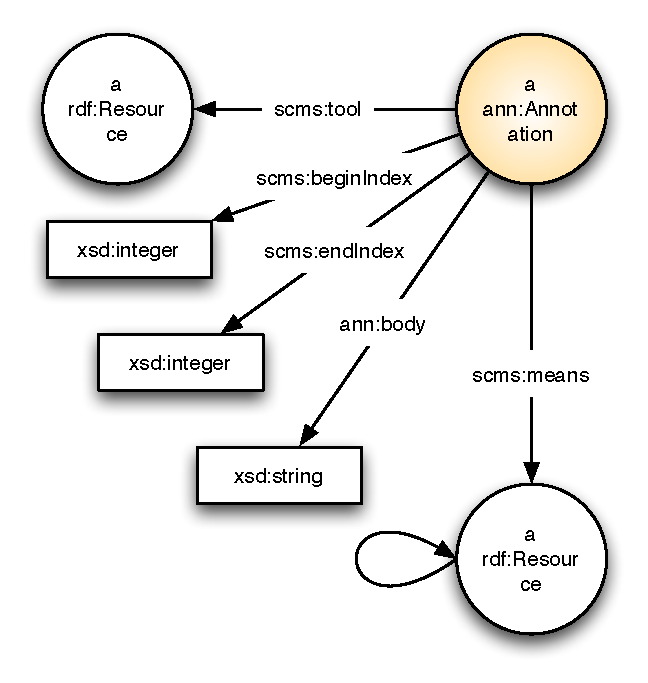
\includegraphics[scale=0.50]{images/NEAnnotation}
}\qquad
\subfloat[fig:ke][Keyword Annotation]{
    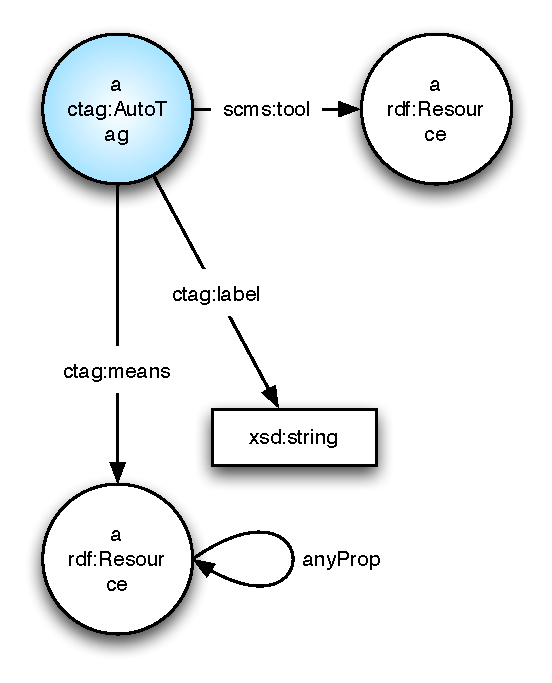
\includegraphics[scale=0.50]{images/KWAnnotation}
}
\caption{Vocabularies used by FOX for representing named entities (a) and keywords (b)}
\label{fig:annotation-vocab}
\end{figure}


\section{Developers' Manual}
\geolift contains three basic \emph{Java} packages: 
\begin{itemize}
 \item \texttt{IO package} which deals with input/output operations using the \emph{Reader} and \emph{Writer} classes.
 \item\texttt{Operators package} will contains implementation of different operators like \emph{merge, split, filter, ...} 
 \\\emph{NOTE: Operators package will be implemented in future version of \geolift}.
 \item\texttt{Modules package} contains the \texttt{GeoLiftModule} interface which is implemented by the basic classes: 
  \texttt{URIDereferencing} class which handles dereferencing  geographical information extending process. 
 \texttt{Linking} class which handles linking geographical information extending processes. 
 and \texttt{nlpEnrichGeoTriples} class which handles named entity extraction process.
\end{itemize}

 All modules implement the \texttt{GeoLiftModule} interface's two methods \texttt{getParameters()} and \texttt{process()},
 where the \texttt{getParameters()} method returns a list of its module input parameters,
 and the \texttt{process()} method takes as input a \emph{Jena} model and a Map of different parameters in form of \texttt{("parameterName", "parameterValue")},
 and as output it generates a Jena model also, this organization ease the usage of the modules in different workflows.

 Moreover, a \emph{Java} jar file is generated for each module, which can be executed directly from command line along with each module parameters.
 
%%%%%%%%%%%%%%%%%%%%%%%%%%%%%%%%%%%%%%%%%%%%%%%%%%%%%%%%%%% Dereferencing Module%%%%%%%%%%%%%%%%%%%%%%%%%%%%%%%%%%%%%%%%%%%%%%%%%%%%%%%%%%%%%%%%%%%%%%%%%%%%%%%%%%%%%%%%
\subsection{Dereferencing module}
 The purpose of the dereferencing module is to extend the model's Geo-spatial information by set of information through specified predicates.

\subsubsection{Input}
\begin{itemize}
 \item \texttt{Data model} contains the triples of the dataset to be enriched 
 (This data model can be an output from previous stage or can be loaded from file/URI directly before using the module). 
 \item \texttt{Predicates list} list of interested predicates to be added as enrichment to the data model.
 Table \ref{tbl:derefPram} provides details about each of the \texttt{URIDereferencing} module's parameters.
\end{itemize}



\begin{table*}[ht]
\caption{Dereferencing parameters description} \label{tbl:derefPram}
\begin{tabular}{@{}  l  l p{7cm} l p{6cm}@{}}
\toprule
\textbf{Parameter Name} & \textbf{Default value} & \textbf{Description}\\
\midrule
\texttt{predicates} 	& \texttt{null} 	& List of interesting predicates to enrich the model, and their Objects' values.  The predicates are given in form of Map structure where the key is a user-defined name for the predicate and the map value is the predicate itself. e.g. $\langle$``predicate1'',``\url{http://www.w3.org/2003/01/geo/wgs84_pos#lat}''$\rangle$. \\
\bottomrule
\end{tabular}
\end{table*}

\subsubsection{Output}
\begin{itemize}
 \item \texttt{Data model} enriched data model with additional Geo-spatial information added by the given input predicates with its extracted object values.
\end{itemize}

\subsubsection{Process}
 In this module, a \emph{Java Jena} model and a list of interested predicates are given as inputs.
 This is done by iterating over the model's resources (dubbed as original resources) 
 and for each of the original resource an extraction of the predicates' values (objects) that are in the form of URI is performed. 
 These URIs (dubbed as dereferenced resources) are more filtered to be the resources used in \emph{DBpedia}.
 The dereferenced resources are handled by a dereference operation in order to find the interested predicates list for them.
 Such predicates and their objects' values are fetched and added to the the original resource to extend its information.
\subsubsection{Sample code to run the module}
Listing \ref{lst:URIDereference} provides a sample code showing how to use the \texttt{URIDereference} module:\\

\begin{lstlisting}[label=lst:URIDereference, numbers=left, numberstyle=\tiny, caption = Code fragment to call the \texttt{URIDereferencing} class.]
public static void main( String[] args ){	
  String datasetSource="";
  List<String> predicatesLines=null;
  if(args.length > 0){
    for(int i=0;i<args.length;i+=2){
      if(args[i].equals("-d") || args[i].equals("--data"))
	datasetSource = args[i+1];
	if(args[i].equals("-p") || args[i].equals("--predicate"))
	  predicatesLines= getConfigurations(args[i+1]);
	}
    }
    try{ 
      Model model=org.aksw.geolift.io.Reader.readModel(datasetSource);//First parameter: model is loaded with dataset from specified file/endpoint
      //Collect list of targeted predicates into Map
      Map<String, String> parameters= list2map(predicatesLines);
      //create Dereferencing object to start the process
      URIDereferencing u = new URIDereferencing();
      // run the dereferencing process it requires model contains the dataset and list of targeted predicates to enrich the model
      Model resultedModel = u.process(model, parameters);
      resultedModel.write(System.out,"TTL");
    } catch (Exception e) {
      e.printStackTrace();
      }
}

\end{lstlisting}

The dereferencing module can be also directly executed from command line using the provided \texttt{dereferencing.jar} file.
The following example introduce calling it to enrich the \emph{Berlin DBpedia} resource with additional predicates located at \texttt{predicatesList.txt} file.

{\flushleft\texttt{java -jar dereferencing.jar -d \url{http://dbpedia.org/page/Berlin} -p predicatesList.txt}}

%%%%%%%%%%%%%%%%%%%%%%%%%%%%%%%%%%%%%%%%%%%%%%%%%%%%%%%%%%% Linking Module%%%%%%%%%%%%%%%%%%%%%%%%%%%%%%%%%%%%%%%%%%%%%%%%%%%%%%%%%%%%%%%%%%%%%%%%%%%%%%%%%%%%%%%%

\subsection{Linking module}

\subsubsection{Input}
\begin{itemize}
 \item \texttt{Data model} contains the triples of the dataset to be enriched 
 (This data model can be an output from previous stage or can be loaded from file/URI directly before using the module). 
 \item \texttt{Parameters list} that will be used during the process. These parameters include:
 \subitem \texttt{Specification file path}, the path to the \texttt{spec.xml} file contains the linking specifications
 \subitem \texttt{URI position}, represents the original model's URI position as source or target in the linking specifications.
\end{itemize}
The parameters, other than the data model parameter, are  collected in Map structure form,
where each entry's value in the Map represents the parameter itself.
Table \ref{tbl:linkingPram} provides details about the \texttt{Linking} module's parameters .
\begin{table*}[ht]
\caption{Linking parameters description} \label{tbl:linkingPram}
\begin{tabular}{@{}  l  l p{7cm} l p{6cm}@{}}
\toprule
\textbf{Parameter Name} & \textbf{Default value} & \textbf{Description}\\
\midrule
\texttt{Specification file} 	& \texttt{N/A} 	& The path to specification file used for linking process, the original dataset to be enriched must be on the source dataset , e.g. \url {linkingModuleData/linking/spec.xml}. The parameter's entry in th Map structure has key 'specFilePath'.\\
\texttt{Links file} 	& \texttt{N/A} 	& The path to links file resulted from the linking process. This file's path is the same as the one specified in LIME's specifications file as output file, e.g. \url {linkingModuleData/linking/links.nt}. The parameter's entry in th Map structure has key 'linksFilePath'.\\
\texttt{Original URI position} 	& \texttt{N/A} 	& represents the original model's URI position as source/left or target/right in the linking specifications. Its value is either 'source' or 'target'. The parameter's entry in th Map structure has key 'linksPart'.\\ 
\bottomrule
\end{tabular}
\end{table*}
\subsubsection{Output}
\begin{itemize}
 \item \texttt{Data model} enriched with additional geographic information URIs represented in \texttt{owl:sameAs} predicates.
\end{itemize}

\subsubsection{Process}
In this module an input model is given and list of parameters for used files during the process. The process starts by generating links between the dataset model and another dataset as second partner. 
This is done using LIMES link discovery framework by specifying the linking specification file given as parameter.
The links are generated in \texttt{accept.nt} file that is used after to combine such links with their original resources in the source dataset model as \texttt{owl:samAs} predicates objects. The result is a dataset model enriched with geographical information links. 
Another forward step is to feed the Dereference module with the resulted enriched model from Linking module as input. 
The previously generated links in the model in addition to other objects in the URIs form will be dereferenced adding more and detailed geographical information.
\subsubsection{Sample code to run the module}
Listing \ref{lst:Linking} provides a sample code showing how to use the Linking module.
\begingroup
    \fontsize{8pt}{10pt}\selectfont
\begin{lstlisting}[label=lst:Linking, numbers=left, numberstyle=\tiny, caption = Code fragment to call the \texttt{Linking} class.]
public static void main(String[] args){
  Map<String, String> parameters=new HashMap<String, String>();
  String linksPath = "";
  if(args.length > 0){
    for(int i=0 ; i<args.length ; i+=2){
      if(args[i].equals("-d"))
      parameters.put("datasetSource",args[i+1]);
      if(args[i].equals("-s")){
	parameters.put("specFilePath",args[i+1]);
	linksPath = args[i+1].substring(0,args[i+1].lastIndexOf("/"))+"/accept.nt";
	parameters.put("linksFilePath",linksPath);
      }
      if(args[i].equals("-p"))
	parameters.put("linksPart",args[i+1]);
    }
  }
  try{
    Model model = org.aksw.geolift.io.Reader.readModel(parameters.get("datasetSource"));
    Linking l = new Linking();
    model = l.process(model, parameters);
    try{
      File file = new File(linksPath);
      file.delete();
    }catch(Exception e){
	e.printStackTrace();
      }
    model.write(System.out,"TTL");
  } catch (Exception e) {
      e.printStackTrace();
    }
}
\end{lstlisting}
\endgroup
The linking module can be directly executed from command line using the provided \texttt{linking.jar} file.
The following example introduces its execution to enrich loaded dataset from \emph{dataset.ttl} with additional links to another dataset according to specifications in \texttt{spec.xml} file.

{\flushleft\texttt{java -jar linking.jar -d dataset.ttl -s spec.xml -p target}}
%%%%%%%%%%%%%%%%%%%%%%%%%%%%%%%%%%%%%%%%%%%%%%%%%%%%%%%%%%% NLP Module%%%%%%%%%%%%%%%%%%%%%%%%%%%%%%%%%%%%%%%%%%%%%%%%%%%%%%%%%%%%%%%%%%%%%%%%%%%%%%%%%%%%%%%%


\subsection{NLP module}
\subsubsection{Input}
\begin{itemize}
 \item \texttt{Data model} contains the dataset to be enriched 
 (This data model can be an output from previous module or can be loaded from file/URI directly before using the module). 
 \item \texttt{Parameters list} that will be used during the process. The \texttt{getParameters()} method of the \texttt{NlpGeoEnricher} class returns a list of parameters,
 which can be set by the user to provide custom control of the \emph{Named entity extraction} provided by the implemented \emph{FOX framework}.
\end{itemize}

\subsubsection{Output}
\begin{itemize}
 \item \texttt{Data model} enriched with additional Geo-spatial information URIs represented by \texttt{http://geoknow.org/ontology/relatedTo} predicates.
\end{itemize}

\subsubsection{Process}
The \texttt{process()} method of the \texttt{NlpGeoEnricher} class takes as input a \emph{Jena} model and a \texttt{Map} of different parameters, 
and as output it generates a \emph{Jena} model also.
Table \ref{tbl:nlpPram} provides details about the \texttt{NlpGeoEnricher} module's parameters .

\subsubsection{Sample code to run the module}
A sample code showing how to call the \texttt{NlpGeoEnricher} class and giving it its parameters is introduced in Listing \ref{lst:NlpGeoEnricher}.

The Nlp module can be directly executed from command line using the provided \texttt{nlp.jar} file.
The following example introduces its execution to enrich \emph{DBpedia Berlin} resource with additional Geo-spatial data through NLP using the FOX light version (-l true).
The output will be written in the \texttt{enriched.ttl} file.

{\flushleft\texttt{java -jar nlp.jar -i http://dbpedia.org/resource/Berlin -o output.ttl -l true}}

\begin{table*}[ht]
\caption{NLP parameters description} \label{tbl:nlpPram}
\begin{tabular}{@{}  l  l p{7cm} l p{6cm}@{}}
\toprule
\textbf{Parameter Name} & \textbf{Default value} & \textbf{Description}\\
\midrule
\texttt{input} 		& \texttt{N/A} 		& The input file/URI to be enriched\\
\texttt{output} 	& \texttt{N/A} 		& The output file to write the enriched model to it\\

\texttt{litralProperty}	& \texttt{Top Ranked} 	& Literal property used by FOX for NER, if not set the top ranked literal property is pecked by \texttt{LiteralPropertyRanker} module, which ranks the  lateral properties of a model according to the average size of each literal property divided by the number of instances of such property.\\
\texttt{useFoxLight} 	& \texttt{false} 	& Use the light version of FOX, setting it generates faster execution time but less accurate results) \\
\texttt{askEndPoint} 	& \texttt{false} 	& Ask the \emph{DBpedia} endpoint for each location returned by FOX (setting it generates slower execution time but more accurate results)\\
\texttt{foxType} 	& \texttt{TEXT} 	& FOX input type : \texttt{\{ text $\rvert$ url \}}\\
\texttt{foxTask} 	& \texttt{NER} 		& FOX task \texttt{:\{NER\}} for Named Entity Recognition\\
\texttt{foxInput} 	& \texttt{""} 		& FOX actual input as text or an URL\\
\texttt{foxOutput} 	& \texttt{TURTLE} 	& FOX output format: \texttt{\{ JSONLD $\rvert$ N3 $\rvert$ N-TRIPLE $\rvert$ RDF/\{ JSON $\rvert$ XML $\rvert$ XML-ABBREV\} $\rvert$ TURTLE \}}\\
\texttt{foxUseNif} 	& \texttt{false} 	& FOX generates NIF: \{ true $\rvert$ false \}\\
\texttt{foxReturnHtml} & \texttt{false} 	& FOX returns HTML: \texttt{\{ true $\rvert$ false \}}\\ 
\bottomrule
\end{tabular}
\end{table*}

% \newpage

\begin{lstlisting}[label=lst:NlpGeoEnricher, numbers=left, numberstyle=\tiny, caption = Code fragment to call the \texttt{NlpGeoEnricher} class.]
// Define geoEnricher object
NlpGeoEnricher geoEnricher= new NlpGeoEnricher();
// Define parameters Map
Map<String, String> parameters = new HashMap<String, String>();
// Set parameters
parameters.put("useFoxLight", "true");
parameters.put("askEndPoint", "false");
// read input Model
Model inputModel = org.aksw.geolift.io.Reader.readModel(inputFileURI);
// Enrich the Model
Model enrichedModel = geoEnricher.process(inputModel, parameters);
// Use the enriched output model
enrichedModel.write(System.out,"TTL");

\end{lstlisting}
 
% \newpage 
% \clearpage


\section{Conclusions}
In this manual, we presented the \geolift component for enriching RDF datasets with geo-spatial data.
In future work, we aim to implement a graphical user interface on top of \geolift to enable users to specify their workflows graphically.
Moreover, we aim to implement workflow checking functionality.

\bibliographystyle{plain}
\bibliography{limes,literature,bibliography,aksw,references}
\end{document}

